\documentclass[journal]{IEEEtran}
\usepackage{blindtext}

% *** GRAPHICS RELATED PACKAGES ***
\usepackage[pdftex]{graphicx}
\graphicspath{{img/}}
\DeclareGraphicsExtensions{.pdf,.jpeg,.png,.pdf_tex}
\usepackage{color}

% *** MATH PACKAGES ***
\usepackage{amsmath}
\usepackage{amssymb}
\interdisplaylinepenalty=2500

% *** SPECIALIZED LIST PACKAGES ***
\usepackage{algorithmic}

% *** ALIGNMENT PACKAGES ***
\usepackage{array}

% *** SUBFIGURE PACKAGES ***
%\usepackage[caption=false,font=footnotesize]{subfig}
%\usepackage{subcaption}

% *** PDF, URL AND HYPERLINK PACKAGES ***
\usepackage{url}
\usepackage[noadjust]{cite} 
\usepackage{csquotes}
\usepackage[nolist,nohyperlinks]{acronym}
\newcommand{\figref}[1]{\figurename~\ref{#1}}
\newcommand{\tabref}[1]{\tablename~\ref{#1}}

% correct bad hyphenation here
%\hyphenation{}

\begin{document}
% paper title
% can use linebreaks \\ within to get better formatting as desired
\title{Exploring the low level design space \\of back-end services}
%\title{Exploring the design space of self-made back-end services: \\ Or how to lose your mental sanity with C}

\author{\IEEEauthorblockN{Eduardo Rodriguez Fernandez}\\
\IEEEauthorblockA{Chair for Data Processing, Technical University of Munich}\\
\IEEEauthorblockA{\texttt{eduardo.rodriguez@tum.de}}
%\thanks{Nobody}
}

% make the title area
\maketitle

\begin{abstract}
Most of the popular modern web development frameworks, like Node.js and Go, handle the creation and management of a backend service in a mostly abstracted high-level way that does not allow a developer much freedom to modify the inherent system architecture of the server. Such an inflexible and abstracted, often plug-and-play, server implementation helps to facilitate web development by concealing the system-level design choices from the end user. Modern web frameworks mostly try to handle concurrent client connections in user-space under the premise that handling concurrency in kernel-space is too costly. The problem of blindly relying on a web framework without understanding its internal architecture is that it might not be the most efficient choice for a web application that has to deal with multiple concurrent connections. The aim of this paper is to provide an experimental comparison in the CPU utilization efficiency of two completely different concurrency-handling paradigms: a multi-process implementation in C and a \textit{goroutine}-based non-preemptively scheduled web service in Go. In order to see if there is a performance penalty for handling concurrency in web applications primarily in kernel-space, rather than in user-space, as most modern web frameworks tend to do nowadays.
\end{abstract}

% Note that keywords are not normally used for peerreview papers.
\begin{IEEEkeywords}
backend development, concurrency, C, Go, databases, software architecture, systems programming, instant messaging, software engineering
\end{IEEEkeywords}
\section{Introduction}
Describe that a chat app is being used as an example implementation. Argue why the architectural design of the chat app is more IO-bound that CPU-bound \cite{Kennedy2018} and therefore works best with a traditional pre-emptive scheduler.

"If you have a program that is focused on IO-Bound work, then context switches are going to be an advantage. Once a Thread moves into a Waiting state, another Thread in a Runnable state is there to take its place. This allows the core to always be doing work. This is one of the most important aspects of scheduling. Don’t allow a core to go idle if there is work (Threads in a Runnable state) to be done.

If your program is focused on CPU-Bound work, then context switches are going to be a performance nightmare. Since the Thead always has work to do, the context switch is stopping that work from progressing. This situation is in stark contrast with what happens with an IO-Bound workload"\cite{Kennedy2018} (correct this since it is actually from part 1)


\section{State of the art}
As mentioned previously, choosing C as the sole development language is a deliberate design decision, since it provides all possible concurrency primitives natively in Unix systems (threads, message queues, processes, file locks, etc.), while only requiring the standard library. This fact provides as much freedom as possible to experiment and explore diverse concurrent back-end architectures, while also making the code easily portable to all Unix systems.

Arguably, Go is very well suited to be used as a state of the art comparison to this paper's proposed implementation in C. First of all, Go was created at Google in 2010 by some of the computer science pioneers that originally came up with Unix and C at Bell Labs, so it is no surprise that Go has been described as a "C-like language" or as "C for the 21st Century" \cite{GoPL2015}. Furthermore, it was created with "built-in concurrency" to tackle modern large distributed infrastructure problems and it is currently widely used at all network traffic levels as a server side service provider \cite{Pike2012}. Therefore, it is a great candidate as a point of reference of how modern server side network concurrency is handled, from which a totally different architecture based on blocking processes can be developed. 

If the main goal of this paper is to open a developer's eyes to the many different concurrency paradigms that can be used for server side development, then the philosophy of Go (and for that matter, also of other popular frameworks like Node.js) is the antithesis of this work, because these frameworks provide an inflexible architecture that handles concurrency. In the case of Go, the syntax to handle the creation of concurrent workloads (so-called "\textit{goroutines}") and of communication channels between the goroutines is so simple that an unaware or beginner programmer might be completely oblivious of the scheduling work being performed under the hood by the Go runtime, or even of the fact that its code is running concurrently. 

\subsection{Goroutines}
The idiomatic way of dealing with client connections in Go, either in an HTTP server or through solely raw TCP communication, is by spawning a new goroutine that handles each client concurrently \cite{Morsing2013_2}\cite{GoNet}\cite{GoHTTP}. From a software engineering perspective this is a very practical approach. First, it moves the level of abstraction that the programmer has to deal with to a higher level, where it is unnecessary to directly intervene in memory synchronization and the management of a thread pool. This should have as a consequence gains in developer productivity and a faster development pace through abstraction, with the trade-off that there is less design freedom. The pledge of Go is that the runtime will solely handle the scheduling of goroutines, and that they are so lightweight that the developer should not worry upfront about the amount of goroutines that would simultaneously be spawned \cite{Cox-Buday2017}.

Goroutines are very lightweight concurrent subroutines  supervised by the Go \textit{runtime} in userspace. Their memory footprint is very small, the assigned memory by default is only a few kilobytes at their creation \cite{Cox-Buday2017}. From the perspective of the kernel goroutines are non-preemptive, i.e. they are not interrupted by the OS scheduler to run other goroutines. They have defined \textit{points of entry} where they can be suspended or activated by the runtime scheduler, which is entirely running in userspace. Since a context-switch between goroutines happens in userspace and the runtime decides which data should be persistent between goroutines, it orders of magniude faster than context-switching between OS threads \cite{Cox-Buday2017} and processes \cite{Kerrisk2010}.

\subsection{Runtime}

-----------------------------------

If, another main discussion in the methodology would be the async own database implementation, it would be interesting to talk about locks in any db system, and use the data book as a major reference.

Might as well read and describe how nginx works ?????

\section{Problem statement}
As previously stated in the introduction, there is ample literature that affirms that kernel-space context-switching in multi-procedural programs should have a worse CPU-utilization performance than user-space context-switching, but none of the bibliographic sources provide experimental data to corroborate this, show how big the difference is or perform a benchmark for network-related concurrency handling \cite{2003Events}\cite{2005Threads}\cite{2013ContextSwitching}\cite{Cox-Buday2017}\cite{Kerrisk2010}.

This work strives to first design the architecture of a multi-procedural concurrent IM application written in C and, then, create a benchmark that makes a performance comparison with a non-preemptively scheduled IM application in Go possible, to address the following research questions (RQ):

\textbf{RQ 1: How does the mean CPU usage of a multi-procedural C application compares to the CPU usage of a non-preemptively scheduled executable in Go?} As an experimental comparison of the performance of context-switching with a user-space paradigm and a kernel-space one.

\textbf{RQ 2: How stable over a period of time is the CPU usage of the two models being compared?} Is there a difference in the coefficient of variation of both concurrency models? This question is important to more accurately provision servers for high load scenarios.

\textbf{RQ 3: How portable across Unix platforms is the IM application developed in C with minimal dependencies?}

How do two different concurrency approaches like processes and goroutines compare performance-wise (CPU utilization) with a same implementation?




\section{Implementation}
%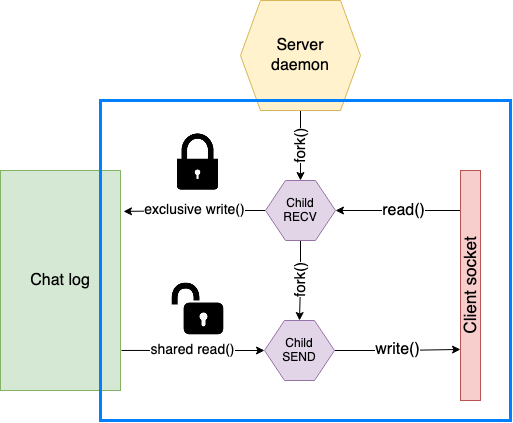
\includegraphics[width=1in,height=1.25in,keepaspectratio]{img/server.png}
\begin{figure}[!t]
	\centering
	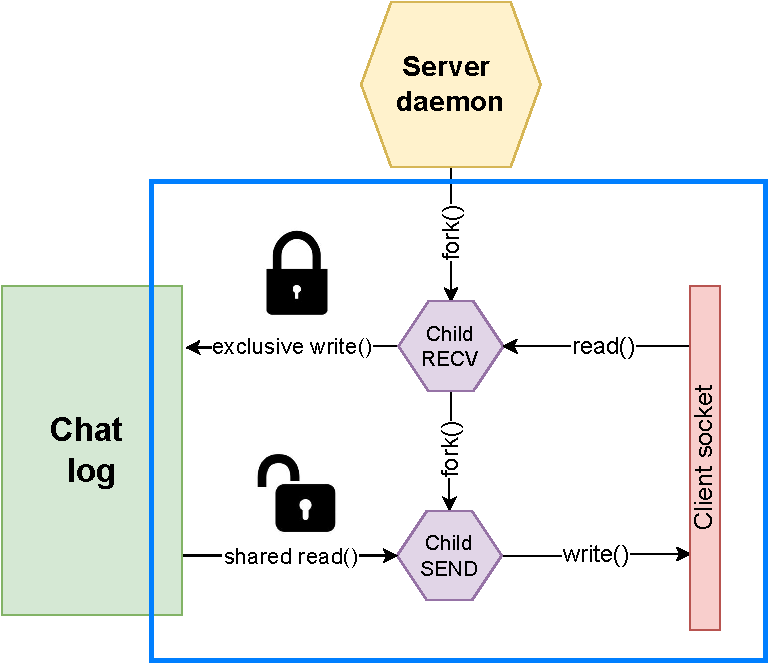
\includegraphics[width=2.5in]{img/server.pdf}
	%where an .eps filename suffix will be assumed under latex, 
	%and a .pdf suffix will be assumed for pdflatex; or what has been declared
	%via \DeclareGraphicsExtensions.
	\caption{Server's back-end architectural overview. The blue rectangle denotes the process cluster created exclusively for each client taking part in a chat service.}
	\label{fig_server_backend}
\end{figure}
The requirements for the chat application are that an undefined number of participants can simultaneously exchange text messages in a chatroom. Furthermore, the communication might be asynchronous, so that the participants can read messages sent to them while they were not connected to the server. The application should use the least amount of dependencies as possible to enable portability across Unix systems, i.e. the chat server should compile natively to FreeBSD or a Linux distribution with the same source file.

The server fundamentally requires a process working as a daemon accepting incoming connection attempts from clients. For each accepted client connection there are multiple possibilities regarding the architecture of the server. The daemon could handle each client separately in a unique thread or child process.

The server will mostly have an IO-bound workload, consisting of handling asynchronous network packets and writing the messages from the users into files in the server's filesystem. An IO-bound workload benefits from the use of a pre-emptive scheduler, since the threads or processes are constantly changing alternatively between a blocked and an unblocked state in an unpredictable manner. As soon as a client goes silent the pre-emptive scheduler can run any other runnable process \cite{Kennedy2018}. Hence, the context-switching is actually advantageous for IO-bound workloads, whereas in CPU-bound workloads (e.g. intensive long-running sequential computations) it becomes a performance bottleneck.

Therefore, handling each client connection separately by forking a child process seems like a good fit for the kind of workload that is expected. Nonetheless, it must be acknowledged that a counterargument against using processes is that thread creation and context-switching times are generally faster than for processes, since processes have an inherently more complex memory layout than threads \cite{Kerrisk2010}.

However, other reasons settled the decision towards processes instead of threads. Before going into these reasons, it makes sense to review the architecture that was actually implemented as a solution. Figure \ref{fig_server_backend} shows a high-level representation of how the server handles every client connection. After successfully authenticating a client, the server daemon calls the \textit{fork} syscall and creates a new child process exclusively for the new client.
 
This child process, called "\textit{Child RECV}" in fig. \ref{fig_server_backend}, inherits a copy of the newly established socket which handles the client. Child RECV is responsible for reading any incoming messages from the client, writing these messages in a concurrently-safe way into a central chat log, sending a multicast signal to let all other clients know that there is a new message and creating a further child process called "\textit{Child SEND}". \textit{Child SEND} also inherits the client's socket in order to send the messages stored in the central chat log at an appropriate time to the client. The blue rectangle depicted in figure \ref{fig_server_backend} comprises a single process cluster for a particular client. For every client connected simultaneously to the server there is one of this process clusters running concurrently.

 Compartmentalizing the different clients into separate processes has the intrinsic advantage of granting more availability in case of a distributed denial of service (DDoS) attack or simply heavy traffic in the server's public-facing daemon. If for any reason, the daemon is getting cluttered with connection attempts, to a point in which the high load threatens to affect the communication performance of the clients already participating inside a chat service, then the daemon's process can be temporarily stopped, or even killed, so that the public-facing port is closed. Since each client's process cluster works completely independently from the daemon accepting new clients and from all other clients' process clusters, the service can continue uninterrupted for all clients already connected. 
 
 From a system administration perspective it is also very convenient to handle each client connection with different processes, since it makes the monitoring and administration of system resource utilization in a \textit{per-client} granular way easy through the use of command line tools like \textit{kill}, \textit{ps}, \textit{ss} or \textit{sockstat}, and \textit{top}.

\subsection{Transactional isolation and atomicity}
Although the data model of the chat application would fit well within a relational database, since the types of the data fields for every message exchange are immutable and translatable into the data types used in relational databases, the system intentionally avoids using any kind of external database system. This design decision makes the application more easily portable and deployable, due to the fact that the same executable of the chat server entirely handles the message storing and retrieving for all data exchanges. Deploying the chat server into a cloud server is as easy as pulling the repository, compiling and running the binary, there is no need to first install and configure a (No)SQL server.

Nonetheless, this implies that the chat program has to fulfil some data safety guarantees that would otherwise be outsourced entirely to the database management system (DBMS). Mainstream DBMS have the ability to perform a series of reads and writes to the underlying data system as a single "\textit{logical unit}" \cite{Kleppmann2017}, a so-called "\textit{transaction}". A transaction is useful as a way of ensuring atomicity and isolation within a distributed system.

Since the incoming messages from the clients will all be centrally stored in a log file and messages from different clients can arrive at any time simultaneously to the server, a transactional mechanism is implemented to avoid race conditions. 

Therefore, the data management system must fulfil the following four requirements. Multiple clients simultaneously writing to the log file should not over-write their messages. Furthermore, it should not be possible to read the log file during a write-operation from another client to avoid reading incomplete data, and, conversely, it should not be possible to write to the log, while another client is reading from it. Finally, unlimited concurrent reading operations from multiple clients are permitted on the log file, since reading from the log file does not have any side effects on the stored data.

To satisfy these criteria, the server creates and opens the central log file with the "\textit{O\_APPEND}" flag (append mode), so that before each write to the file the offset is positioned at the end of the file and the write operation is subsequently performed in a single atomic operation \cite{Kerrisk2010}. Thus, old data written to the log cannot get corrupted by new writes to the file.

Moreover, a file locking system is implemented using the \textit{flock} syscall, in order to fulfil the previously mentioned four requirements. Two different types of locks can be placed on a file: a shared lock and an exclusive lock. When multiple clients try to simultaneously send messages to the chat log, the child process Child RECV tries to place an exclusive lock on the chat log file.  If no other lock is currently placed on the file, Child RECV can write exclusively into the chat log until the placed lock is released. Meanwhile, no other process can write or read from the file, the other Child RECV processes trying to write to the chat log file would block on the call to flock, until the process holding the exclusive lock releases it. All the necessary writes to the chat log file would be scheduled sequentially.

Conversely, when the server sends new messages to a client through Child SEND, it has to read the messages from the chat log. Hence, the child process places a shared lock on the chat log and reads from it. Any other process trying to simultaneously read from the same file can place another shared lock and read from the file, but a process trying to write to the file would block when placing the exclusive lock, until all shared locks have been released. 

This file handling architecture makes sending messages to multiple clients a highly parallelizable operation, while writing to the chat log is a secure isolated task performed in an atomic way.

\subsection{Multicasting}
The system should deliver new messages instantly through the respective Child SEND process of every client each time a new message is received, in other words, every message must be multicasted to all participating clients. The number of connected clients can change over time and it is unlimited. 

The two main IPC (inter-process communication) mechanisms capable of multicasting to multiple processes are sockets and signals \cite{Kerrisk2010}. Signals are used in this implementation, because from a software engineering perspective configuring sockets to handle multicasting is less portable and requires more code-refactoring.

The Unix standard \textit{SIGUSR1} signal, which is reserved for "user defined behaviour", can be used to synchronously inform a group of processes about an event, in this case, the need to send new messages to the clients.

By choosing to multicast with signals the possibility to work with threads, instead of with processes, was eliminated. Since all threads in a process share the same signal dispositions and for this design different signal disposition between parent and child processes are a requirement. Moreover, this architecture does not require an administrative centralized process constantly monitoring which clients are currently online, to whom the messages should be delivered. Instead, it outsources this task ti the kernel which manages signal distribution.


\subsection{Portability issues}
Even when using only POSIX compliant syscalls the server does not compile entirely the same in all platforms. Mention problem between Debian (Ubuntu and Kali) distributions, in which strace had to be used to pinpoint a compilation difference.

\subsection{Security}
The chat server runs as a long-lasting daemon, therefore leaving at least one port open to the public internet, from which the clients will establish a connection with the server. It must be taken for granted that the open port will eventually be discovered by web-scanning botnets that periodically scan targeted hitlists (specially know IP ranges from cloud providers) or random IP ranges \cite{Mirkovic2004}\cite{Graham}.

We are not containerizing the application, since it would not do it portable across many Unix systems, e.g. the BSDs, so we have to guarantee the security of running an application with an Internet facing open port. -> Authentication system and running the server through a system user with very limited permissions.
The system user technique limits the amount of damage that could possibly be generated, because the system user should not  have that many permissions.

\cite{Kerrisk2021}

--------------------------------------

Mention that there were also portability issues, and that a different behaviour between the development environment and the production or deployment environment was seen. A system call was been compiled differently (the default flags were being used, which where different between systems) so working entirely with gcc and the the standard C library is not a guaranty for automatic perfect portability. In fact, it was very cumbersome to debug the faulty behaviour, since it had to be done using strace, in order to find the misbehaving syscall. Conclusion, thinking that using only C, gcc and the stdlib is working almost dependency-free is a fallacy or an illusion, debugging unexplained behaviour will still be arduous.
\section{Conclusion}
Creating a backend service from the ground up gives the developer the freedom of choosing between a thread-oriented, process-oriented, pre-emptively or non-pre-emptively scheduled architecture. For some applications that are expected to work at almost the full capacity of the CPU usage of a machine, it makes sense to consider porting their code to a multi-process implementation in C, instead of developing in a platform with a more modern and complex concurrency paradigm, like Go. Since, the results of our measurements show a more stable CPU utilization in the multi-procedural implementation in C, with a much lower coefficient of variation under high loads.  Nonetheless, it must be acknowledged that the development productivity while programming low-level network concurrency, as in C, is not as high as compared to a high-level framework with mature networking libraries.

Furthermore, at all levels of concurrent network connections tested, the C implementation with context-switching in kernel-space, instead of in user-space as with the Go application, had a significantly lower percentage of CPU utilization. The non-preemptively scheduled Go application shows an almost linear increase in the CPU utilization proportional to an increase in the number of concurrent connections, while the C program drastically reduces the rate of CPU usage increase after 16 concurrent client connections. In a comparison based on programs similar to real-life deployed network applications, like in this case, the CPU usage is influenced not only by the context-switches, but also by inherent traits of the platform running the application. In this case, the actual performance gains attributable to user-space context-switching dwindle compared to the overhead of the Go runtime and GC.

The dependency restriction of only using the C standard library and compiling with GCC did not guarantee an entirely bug-free portability between Unix platforms. Therefore, even when reducing dependencies to a bare minimum, it is an illusion to think that fully portable code can easily be generated, so that to some extent the appeal and reasoning behind OS-virtualization (container management systems) can be better grasped.

Finally, the software developed in this project \cite{Rodriguez2022}, distributed through a public repository with a AGPL license (GNU Affero General Public License), delivers a functional command-line chat application that gives the user the possibility to self-host its chat service and regain full control over the management of its instant messaging data and metadata. Furthermore, it allows its users to avoid vendor lock-in effects and the single points of failure of an IM application with a centralized architecture like Signal and WhatsApp, since its minimal amount of dependencies facilitate a prompt native deployment in any Unix system.
%\appendices
\section{Proof of the First Zonklar Equation}
Some text for the appendix.

\bibliographystyle{IEEEtran}
\bibliography{other/bibliography}
\nocite{*}

%\begin{IEEEbiography}[{
\includegraphics[width=1in,height=1.25in,clip,keepaspectratio]{img/picture}}]{Eduardo Rodriguez}
%is an Electrical Engineering and IT graduate student at TUM.
%\end{IEEEbiography}

\end{document}
